\documentclass[12pt]{exam}
\usepackage[utf8]{inputenc}

\usepackage{amsmath}
\usepackage{amsfonts}
\usepackage{amssymb}
\usepackage{siunitx}
\usepackage{graphicx}
\usepackage{wrapfig}

\usepackage[titles]{tocloft}
\renewcommand{\cftdot}{}

\usepackage{sectsty}
\sectionfont{\Large}
\subsectionfont{\large}
\subsubsectionfont{\normalsize}

\usepackage[]{geometry}
\geometry{letterpaper, margin=1in,tmargin=50pt}

\usepackage{xcolor}
\definecolor{codegreen}{rgb}{0,0.6,0}
\definecolor{codedarkgreen}{rgb}{0,0.3,0}
\definecolor{codegray}{rgb}{0.5,0.5,0.5}
\definecolor{codepurple}{rgb}{0.58,0,0.82}
\definecolor{backcolour}{rgb}{0.95,0.95,0.92}
\definecolor{codedarkgray}{rgb}{0.2,0.2,0.2}
\definecolor{codenavy}{rgb}{0,0,0.5}
\definecolor{backcolor}{rgb}{0.95,0.95,0.95}
\definecolor{codeblack}{rgb}{0,0,0}

\usepackage{hyperref}
\hypersetup{
	colorlinks=true,
	linkcolor=codenavy,
	urlcolor=blue
}

\usepackage{listings}
\lstdefinestyle{mystyle}{
	basicstyle=\ttfamily,
	backgroundcolor=\color{backcolor},   
	commentstyle=\color{codenavy},
	keywordstyle=\color{codeblack},
	numberstyle=\tiny\color{codegray},
	stringstyle=\color{codedarkgreen},
	basicstyle=\ttfamily\footnotesize,
	breakatwhitespace=false,         
	breaklines=true,                 
	captionpos=b,                    
	keepspaces=true,                 
	numbers=left,                    
	numbersep=5pt,                  
	showspaces=false,                
	showstringspaces=false,
	showtabs=false,                  
	tabsize=2
}
\lstset{style=mystyle}

\title{SBFSEM-tools Documentation}
\author{Sara Patterson, Neitz Lab}
\date{\vspace{-5ex}}

\begin{document}
	\maketitle
	\tableofcontents
	\pagebreak
	% ------------------------------------------------- Section -- 
	\section{Introduction}
	% ------------------------------------------------- Section -- 
	SBFSEM-tools is a Matlab toolbox developed for serial EM data and connectomics in the Neitz Lab at University of Washington. While SBFSEM-tools was built around the Viking annotation software, many aspects are quite general and could apply easily to other programs and imaging methods.\\
	SBFSEM-tools imports annotation data through Viking's OData service and parses the results into Matlab data types. This happens behind the scenes so the average user can work with familiar objects (neuron, synapse, etc).\\
	Other features include:
	\begin{itemize}
		\item Single neuron analysis: dendritic field area, dendrite diameter, soma size, stratification, synapse distribution
		\item Group analysis: density recovery profile, nearest neighbor, synapse statistics
		\item 3D volume rendering of polygon annotations and free-form traces over a stack of EM images. 2D projections of dendritic fields.
		\item Generate surfaces from IPL boundary markers, compensate for Z-axis misalignments.
		\item Misc UIs for visualizing EM images and annotations
	\end{itemize}
	% ------------------------------------------------- Section -- 
	\section{Install}
	% ------------------------------------------------- Section -- 
	SBFSEM-tools is available on Github: \href{http://github.com/sarastokes/sbfsem-tools}{sbfsem-tools}. You can either clone the repository or download it as a ZIP file.
	Make sure sbfsem-tools is on your \href{https://www.mathworks.com/help/matlab/ref/addpath.html}{MATLAB path} either by adding the following to your startup file, or running it from the cmd line.
	See Section \ref{matlab101} and \texttt{Tutorial.m} in the main sbfsem-tools folder for more info on setup.
	% ------------------------------------------------- Section -- 	
	\section{RenderApp}
	% ------------------------------------------------- Section -- 
	\begin{wrapfigure}{r}{0.35\linewidth}
		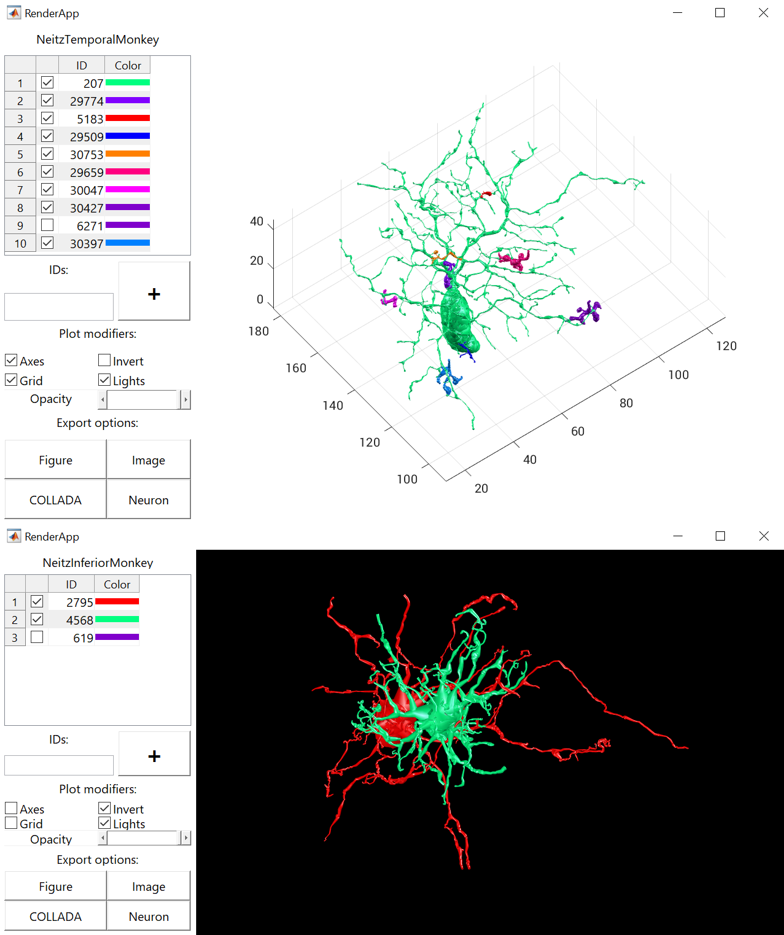
\includegraphics[width=\linewidth]{renderapp}
	\end{wrapfigure}
	RenderApp includes most of the methods relating to 3D rendering but requires minimal interaction with the command line. To get started type:
	\begin{lstlisting}[language=matlab]
	RenderApp();\end{lstlisting}
	The user interface was roughly based on VikingView. 
	The left panel is the user interface panel:
	\begin{itemize}
		\item The volume name is displayed at the top of the left panel.
		\item Each neuron will appear as a line in the table at the top of the left panel. This table offers two controls:
		\begin{itemize}
			\item The checkboxes toggle visibility of the render. This way you can temporarily hide renders without having to reload the neuron later.
			\item Click on the color bar to open a UI for changing the render colors.
		\end{itemize}
		\item Input neuron IDs to the edit box under \texttt{IDs}, and press the \texttt{$+$} button to add them. Add multiple neurons by separating their ID numbers with commas. The loading status of the render will be printed to the command line.
		\item The plot modifiers include:
		\begin{itemize}
			\item \textbf{Axes} - Show/hide the axes.
			\item \textbf{Grid} - Show/hide the grid.
			\item \textbf{Invert} - Switch the background colors from white to black
			\item \textbf{Lights} - Turn the figure lighting on and off. When off, the render will look like a 2D projection.
			\item \textbf{Opacity} - Control the render transparency.
		\end{itemize}
		\item The export options:
		\begin{itemize}
			\item \textbf{Figure} - Open the renders in a new Matlab figure.
			\item \textbf{COLLADA} - Export the renders as a .dae file for Blender.
			\item \textbf{Image} - Save the render as an image (either .png, .jpeg or .tiff).
			\item \textbf{Neuron} - Send the Neuron objects to the base workspace to interact with through the command line.
		\end{itemize}
	\end{itemize}
	The right panel is the render display figure. By clicking anywhere on the render figure, you enable the following keyboard controls:\\
	\begin{center}
	\begin{tabular}{|l l|}
		\hline
		\textbf{KEY} & \textbf{FUNCTION}\\
		\hline
		\texttt{h} & Opens help box\\
		\texttt{c} & Copies Viking location of last mouse click.\\
		\texttt{m} & Return to original axis scaling\\
		\hline
		\textbf{Rotate} & \\
		\texttt{$\leftarrow$} & Decrease azimuth\\
		\texttt{$\rightarrow$} & Increase azimuth\\
		\texttt{$\downarrow$} & Decrease elevation\\
		\texttt{$\uparrow$} & Increase elevation\\
		\hline
		\textbf{Zoom} & \\
		\texttt{z} & Zoom\\
		\texttt{Z} & Hit once to change the zoom direction\\
		\hline
		\textbf{Pan} & \\
		\texttt{a} & Decrease the x-axis\\
		\texttt{d} & Increase the x-axis\\
		\texttt{q} & Decrease the y-axis\\
		\texttt{e} & Increase the y-axis\\
		\texttt{s} & Decrease the z-axis\\
		\texttt{w} & Increase the z-axis\\
		\hline
	\end{tabular}
	\end{center}
	
	The biggest difference is that RenderApp does NOT include synapses. Personally, I always have child structures turned off in VikingView - I'll get around to adding them eventually, but if this is a priority for you, let me know.
	% ------------------------------------------------- Section -- 	
	\section{Neuron}
	% ------------------------------------------------- Section -- 
	Most work revolves around the Neuron class, which is a basic representation of a neuron (called a `Structure' in Viking). A Neuron is created with two inputs: the Structure ID and the volume name. The Neuron class imports the data from Viking's OData service (so you will need internet access).
	\begin{lstlisting}[language=matlab]
	% Cell 6800 from NeitzTemporalMonkey
	c6800 = Neuron(6800, 't');
	% Cell 2795 from NeitzInferiorMonkey
	c2795 = Neuron(2795, 'NeitzInferiorMonkey');
	% Same cell but using the abbreviated volume name
	c2795 = Neuron(2795, 'i');
	
	% Import a neuron with synapses
	c6800 = Neuron(6800, 't', true);
	% Add the synapses to an existing neuron
	c2795.getSynapses();\end{lstlisting}
	The full volume names are: `NeitzTemporalMonkey', `NeitzInferiorMonkey' and 'MarcRC1'. These can be abbreviated to 't', 'i' and 'r', respectively.
	% -----------------------------------------------Subsection -- 
	\subsection{Neuron Properties}
	% -----------------------------------------------Subsection -- 
	Neuron has the following publicly accessible properties:
	\begin{enumerate}
		\item \texttt{viking} - struct - cell info from Viking
		\item \texttt{nodes} - table - all annotations 
		\item \texttt{edges} - table - links between annotations
		\item \texttt{volumeScale} - vector - units are nm/pix for X and Y, nm/section for Z.
		\item \texttt{synapses} - table - all child structures
		\item \texttt{geometries} - table - closed curve geometries
		\item \texttt{analysis} - containers.Map - keys for each NeuronAnalysis
		\item \texttt{model} - a 3D model of the neuron
		\item \texttt{lastModified} - datestr - last update of neuron from OData
	\end{enumerate}
	% -----------------------------------------------Subsection -- 
	\subsection{Neuron Methods}
	% -----------------------------------------------Subsection -- 
	The Neuron class has the following publicly available methods. Most are convenience functions to simplify data access.\\ Type \verb|help Neuron\methodname| for more information on each method. Most are also addressed later in the documentation.
	\begin{enumerate}
		\item \textbf{update}\\
		\textit{Description:} Updates the underlying data from OData. Useful when working with a neuron you are currently annotating.\\
		\textit{Syntax:} \texttt{obj.update();}
		%
		\item \textbf{getSynapses}\\
		\textit{Description:} Import the synapses (`child structures') from OData.\\
		\textit{Syntax:} \texttt{obj.getSynapses}
		%
		\item \textbf{getGeometries}\\
		\textit{Description:} Retrieve closed curve annotation control points from OData - helpful when you need to update frequently but don't want to reload the entire cell.\\
		\textit{Syntax:} \texttt{obj.getGeometries();}
		%
		\item \textbf{build}\\
		\textit{Description:} Create a 3D model (saved to obj.model). Available render types are cylinder (default), closedcurve and disc.\\
		\textit{Syntax:} \texttt{obj.build(renderType)};
		%
		\item \textbf{graph}\\
		\textit{Description:} Convert the neuron into an undirected or directed graph. For more information on what this enables, see MATLAB's \href{https://www.mathworks.com/help/matlab/graph-and-network-algorithms.html}{graph class documentation}.\\
		\textit{Syntax:} \texttt{G = obj.graph();}
		% 
		\item \textbf{render}\\
		\textit{Description:} Render the neuron's 3D model.\\
		\textit{Syntax:} \texttt{obj.render(`ax', axisHandle, `FaceColor', rgb);}
		%
		\item \textbf{printSyn}\\
		\textit{Description:} Print a summary of the neuron's synapses to the command line.\\
		\textit{Syntax:} \texttt{obj.printSyn;}
		\item \textbf{synapseNames}\\
		Outputs a list of synapse types associated with the neuron\\
		\textit{Syntax:} \texttt{names = obj.synapseNames;}
		%
		\item \textbf{getCellNodes}\\
		The node table contains both synapse and cell body annotations. This method returns only the cell body annotations.\\
		\textit{Syntax:} \texttt{T = obj.getCellNodes;}
		%
		\item \textbf{getSynapseNodes}\\
		Same idea as getCellNodes, returns only the synapse annotations.\\
		\textit{Syntax:} \texttt{T = obj.getSynapseNodes(onlyUnique);}
		%
		\item \textbf{getSynapseXYZ}\\
		Returns the XYZ locations of all annotations associated with a given synapse.\\
		\textit{Syntax:} \texttt{xyz = getSynapseXYZ(`synapseName')};
		%	
		\item \textbf{getCellXYZ}\\
		Returns the XYZ locations of all cell body annotations\\
		\textit{Syntax:} \texttt{xyz = obj.getCellXYZ;}
		%
		\item \textbf{synapseIDs}\\
		Returns the location IDs for annotations of a given synapse type.\\
		\textit{Syntax:} \texttt{IDs = obj.synapseIDs(`synapseName');}
		%
		\item \textbf{saveNeuron}\\
		The speed of the OData import should make saving Neurons unnecessary, however, this is an option just in case.\\
		\textit{Syntax:} \texttt{obj.save();}
	\end{enumerate}
	% -----------------------------------------------Subsection -- 
	\subsection{NeuronGroup} 
	% -----------------------------------------------Subsection --
	% -------------------------------------------------- Figure -- 
	\begin{wrapfigure}{r}{0.15\linewidth}
		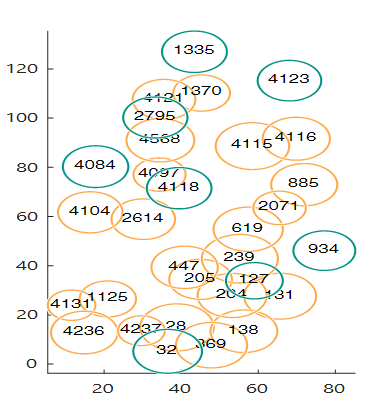
\includegraphics[width=\linewidth]{h1h2mosaic}
	\end{wrapfigure}
	% -------------------------------------------------- Figure -- 
	A single data object to hold related Neurons. Inputs can be ID numbers or existing Neurons.
	\begin{lstlisting}[language=matlab]
	h1hc = sbfsem.NeuronGroup([28, 447, 619]);\end{lstlisting} 
	The NeuronGroup class is still a work-in-progress. The current methods include:
	
	\paragraph{somaPlot} Plot the mosaic of somas
	\begin{lstlisting}[language=matlab]
	h1hc.somaPlot();
	h1hc.somaPlot('addLabel',true); % Label with ID
	h1hc.somaPlot('ax',gca); % Add to existing axis
	% Two methods for controlling plot color:
	h1hc.somaPlot('Color', [0 0.8 0.3]);
	h1hc.setPlotColor([0 0.8 0.3]); h1hc.somaPlot;\end{lstlisting}
	\paragraph{getSomaSizes} Return statistics on the soma sizes. If the NeuronGroup contains cells without annotated somas, set validateSizes = true to exclude them from the analysis.
	\begin{lstlisting}[language=matlab]
	% output = NeuronGroup.somaDiameter(validateSizes);
	x = h1hc.somaDiameter();
	% Catch neurons without annotated somas
	x = h1hc.somaDiameter(true);
	\end{lstlisting}
	
	% -----------------------------------------------Subsection -- 
	\subsection{NeuronAnalysis}
	% -----------------------------------------------Subsection -- 
	The NeuronAnalysis class helps keep population data organized by managing input parameters and results of common analyses. To create a new analysis, subclass NeuronAnalysis and edit the \texttt{doAnalysis} and \texttt{visualize} methods.\\
	See \texttt{Tutorial.m} for information on these existing analysis classes:
	\begin{itemize}
		\item \textbf{DendriticFieldHull} - uses convex hull to estimate dendritic field area, includes methods for removing axons prior to analysis.
		\item \textbf{PrimaryDendriteDiameter} - returns the median dendrite diameter at a given distance from the soma.
	\end{itemize}
	% ------------------------------------------------- Section -- 
	\section{Views}
	% ------------------------------------------------- Section -- 
	Neurons can be passed to several UIs with the following syntax:
	\begin{lstlisting}[language=matlab]
	% Import a neuron with synapses
	c6800 = Neuron(6800, 't', true);
	% Pass the neuron to each view
	NodeView(c6800);
	StratificationView(c6800);
	SomaDistanceView(c6800)\end{lstlisting}
	\begin{itemize}
		\item \textbf{NodeView} - 3D scatter plot of cell and synapse annotations associated with a cell.
		\item \textbf{StratificationView} - Z-axis histogram of dendrites and synapses.
		\item \textbf{SomaDistanceView} - proxmial-distal distribution of dendrites and synapses.
	\end{itemize}
	% -------------------------------------------------- Figure -- 
	\begin{center}
		\begin{figure}[h]
		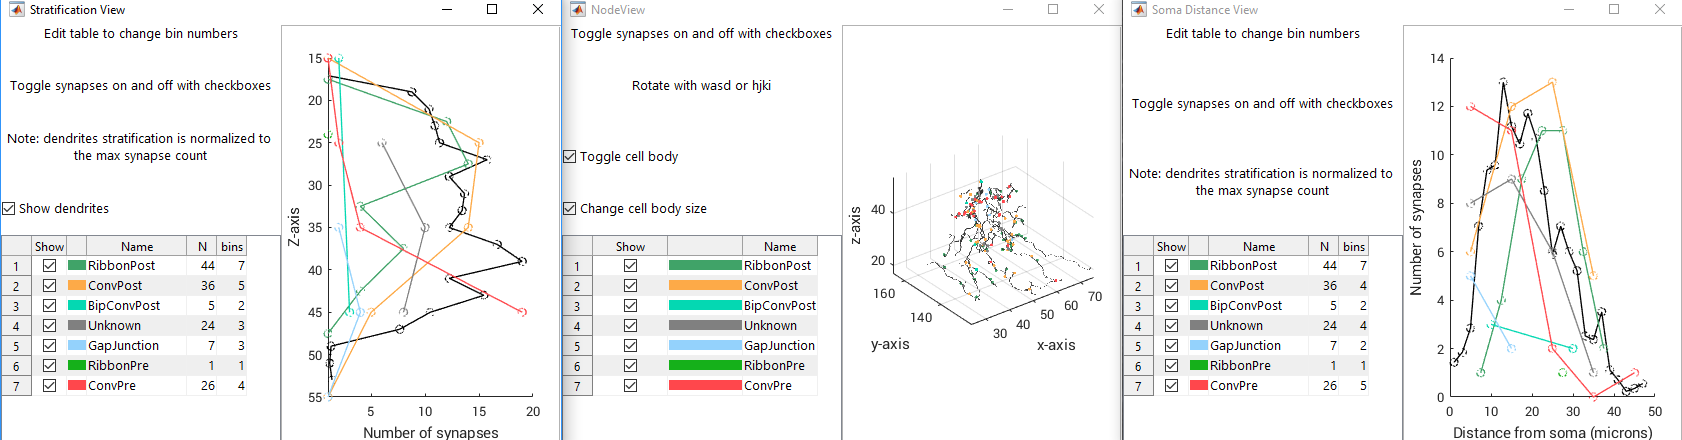
\includegraphics[width=0.95\textwidth]{views}
		\end{figure}
	\end{center}
	% -------------------------------------------------- Figure -- 
	The checkboxes in the synapse table allow toggling the visibility of each synapse type. If the bin numbers in the synapse table are edited, the histogram plots will automatically update.
	% ------------------------------------------------- Section -- 
	\section{Images}
	% ------------------------------------------------- Section -- 
	% -------------------------------------------------- Figure -- 
	\begin{wrapfigure}{r}{0.2\linewidth}
		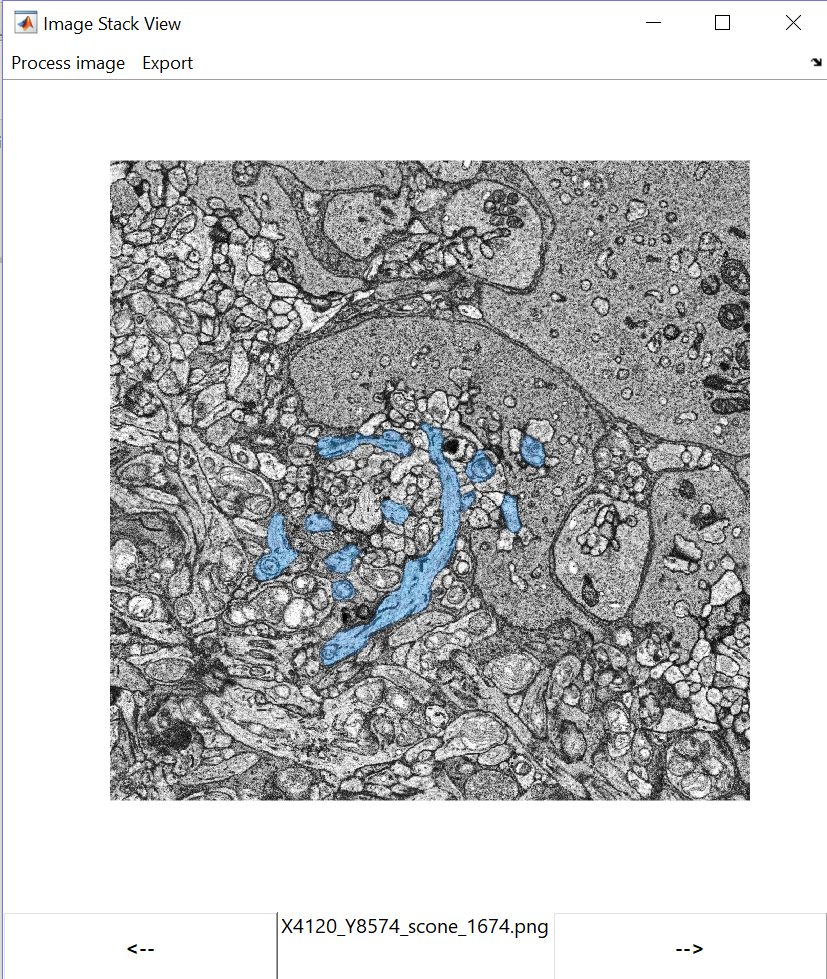
\includegraphics[width=\linewidth]{imstackapp}
	\end{wrapfigure}
	% -------------------------------------------------- Figure -- 
	% -----------------------------------------------Subsection -- 
	\subsection{ImageStackApp}
	% -----------------------------------------------Subsection -- 
	The ImageStackApp was built to scan through a series of images exported using Viking's Export Frames option (although this will work with any folder of images, provided there is some numbering in the file names). Pass a folder name to browse through the images (using left and right arrow keys or buttons). If the filenames contain numbers (Viking's export frames appends a frame number automatically), these will be used to order the images.
	\begin{lstlisting}[language=matlab]
	ImageStackApp('C:\...\foldername');\end{lstlisting}
	To crop the set of images, use \texttt{Process Image $\rightarrow$ Crop} and draw a rectangle on the image. Use \texttt{Full size} to return to the original size. Both changes require moving to another image to apply.
	
	The ImageStackApp creates an ImageStack object. To create a GIF, create an instance of ImageStack alone and use the \texttt{stack2gif} function. 
	\begin{lstlisting}[language=matlab]
	I = sbfsem.images.ImageStack('C:\...\foldername');
	I.stack2gif();\end{lstlisting}
	% -----------------------------------------------Subsection -- 
	\subsection{Image Segmentation}
	% -----------------------------------------------Subsection -- 
	% --------------------------------------------Subsubsection -- 
	\subsubsection{Color ROIs}\label{colorROI}
	% --------------------------------------------Subsubsection -- 
	% -------------------------------------------------- Figure -- 
	\begin{wrapfigure}{r}{0.22\linewidth}
		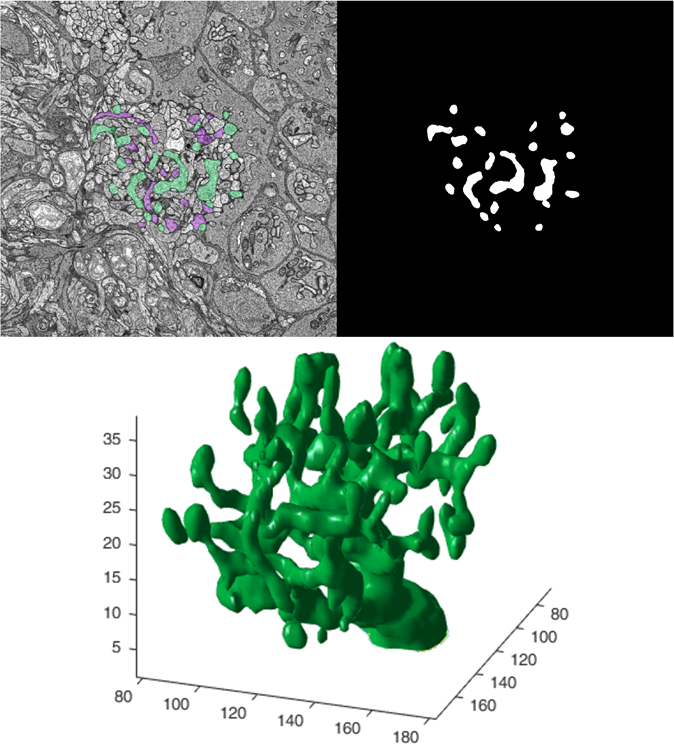
\includegraphics[width=\linewidth]{roi_render}
		\label{colorROI}
	\end{wrapfigure}
	% -------------------------------------------------- Figure -- 
	Renders can also be generated from a stack of EM images with color annotations. See \texttt{algorithms/segmentColorROI.m} for more information. Eventually I will make this more user-friendly. For now, new cell types and their thresholds must be added manually. To the right is an example of an L/M-cone with the ON- and OFF-midgets colored in Photoshop. On the right is the binary matrix output where 1/true (white) indicates a pixel within the color threshold limits.
	\subsubsection{Outlines}
	\texttt{getImageRGB.m} provides a quick tool for extracting data points from an image, given the outlines were drawn with a distinct color (red, green or blue in Paint works just fine). The first argument is the image, the second is the RGB value used to draw outlines.
	\begin{lstlisting}[language=matlab]
	pts = getImageRGB(im, [0 1 0]);\end{lstlisting}
	If more than one outline is present, MATLAB's \texttt{bwboundaries} can probably separate them into distinct objects.
	
	% ------------------------------------------------- Section -- 
	\section{Renders}
	% ------------------------------------------------- Section --
	% -----------------------------------------------Subsection -- 
	\subsection{Polygon Meshes}
	% -----------------------------------------------Subsection -- 

	Unlike the volumetric renders, the polygon meshes retain their absolute XYZ locations. This greatly simplifies the process of rendering multiple neurons to a single scene.
	\begin{lstlisting}[language=matlab]
	% Import a neuron and build the model
	c1441 = Neuron(1441, 'i');
	c1441.build();
	% If no axis handle is provided, creates new figure
	r1441.render();
	% Keep axis handle to direct next render to same figure
	ax = gca; 
	% Import a 2nd neuron and add to render
	c1411 = Neuron(1411, 'i');
	c1411.build();
	r1411.render('ax', ax, 'FaceColor', [0 0.8 0.3]);\end{lstlisting}

	The resulting render is passed through a smooth function automatically. You can bypass this or increase the number of smoothing iterations.\\
	% -------------------------------------------------- Figure -- 
	\begin{wrapfigure}{r}{0.18\linewidth}
		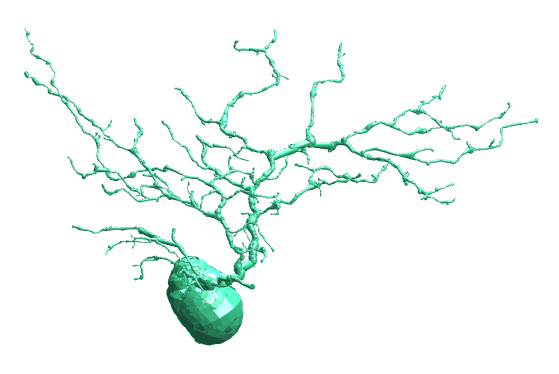
\includegraphics[width=\linewidth]{c6_render}
		\label{c6render}
	\end{wrapfigure}
	% -------------------------------------------------- Figure -- 	
	\begin{lstlisting}[language=matlab]
	% No smoothing
	c121.setSmoothIter(0);
	c121.render();
	% Increase the iterations
	c121.model.setSmoothIter(2); 
	c121.render();\end{lstlisting}
	Surprisingly, increasing the \textbf{smoothing iterations} is typically detrimental. The noise in these renders is resistant to a number of methods, including the standard Laplacian and subdivision smooth functions. I'm working on more advanced methods for smoothing out the renders (and on creating them with less noise in the first place).
	
	You can also set a \textbf{reduction factor} which goes to MATLAB's \texttt{reducepatch} function (\texttt{help reducepatch} for more info). As of 3Jan2017, the current Cylinder algorithm renders show minimal changes with 0.8, 0.9 reduction factors. To visualize the effect:
	\begin{lstlisting}[language=matlab]
	c121 = Neuron(121, 't');
	c121.build();
	c121.model.setReduction(0.8);
	c121.render('reduce', true);\end{lstlisting}
	
	% A brief outline of the steps involved:
	% \begin{enumerate}
	% 	\item Query OData service for the all annotations in a given cell ID. Save the XYZ coordinates, radius and location ID of each annotation. 
	% 	\item Query OData service for all links between annotations.
	% 	\item Apply XY transforms to compensate for major shifts in section alignment.
	% 	\item Query OData service for the volume dimensions - use these to convert XYZ coordinates and radius from pixels to microns.
	% 	\item Convert the annotations and links between each annotation into the nodes and edges of an undirected graph.
	% 	\item Create an undirected graph from all nodes (annotations/locations) and edges (location links).
	% 	\item Use depth-first search (\texttt{dfsearch}) to divide nodes into segments of degree $\le$ 2. This avoids rendering dendrite branches.
	% 	\item Link each segment back to the parent node of degree $>$ 2. This way some nodes are repeated but each edge is represented only once.
	% 	\item Find the magnitude and angle of the distances between all connected nodes. Use this to get a quaternion rotation matrix for each edge.
	% 	\item Input the radii to MATLAB's built-in 3D \texttt{cylinder} function, which creates a cylinder orthogonal to the XY plane.
	% 	\item Rotate each node's cylinder by it's quaternion rotation matrix.
	% \end{enumerate}
	% --------------------------------------------Subsubsection --	
	\subsubsection{Blender Export}
	% --------------------------------------------Subsubsection --
	% -------------------------------------------------- Figure --
	\begin{wrapfigure}{r}{0.3\linewidth}
		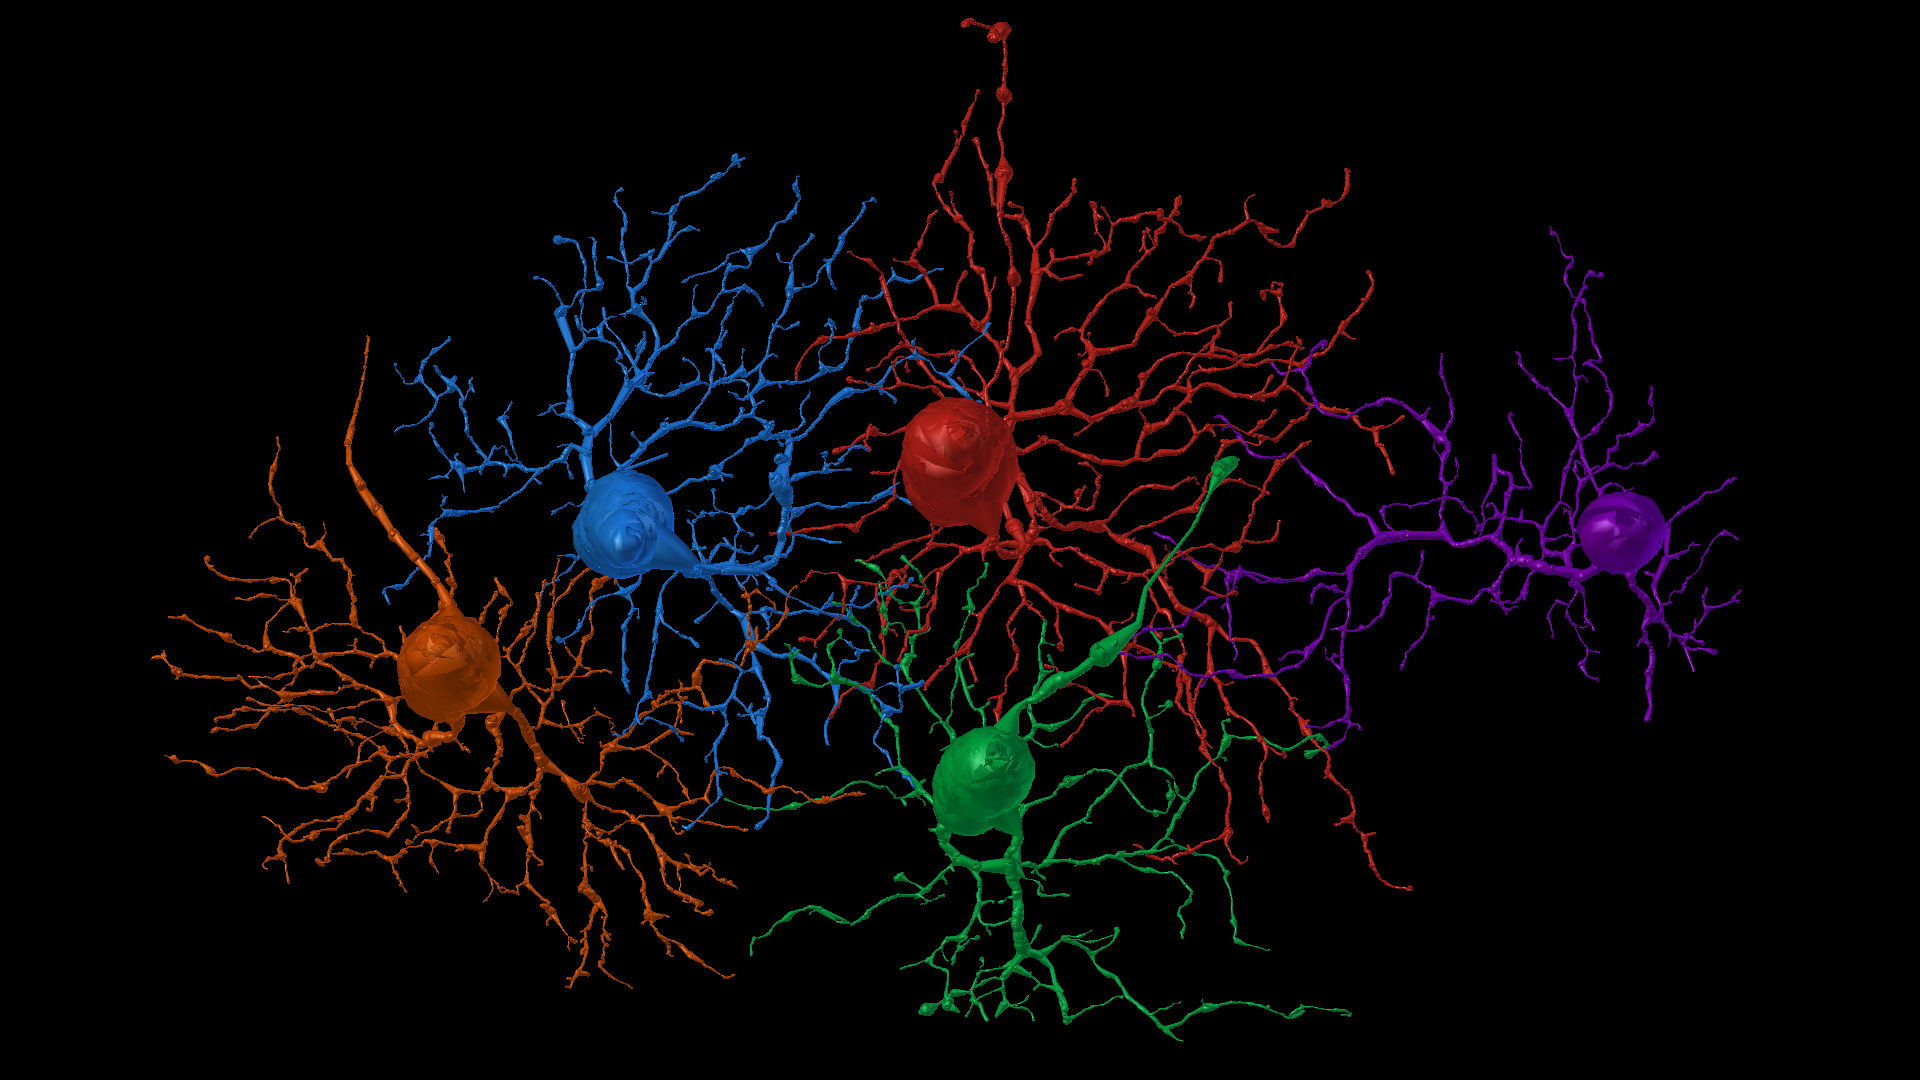
\includegraphics[width=\linewidth]{parasolRGCs}
		\label{blenderParasol}
	\end{wrapfigure}
	% -------------------------------------------------- Figure --
	\paragraph{Single neuron} To export a single neuron to a COLLADA file, use:
	\begin{lstlisting}[language=matlab]
	c619 = Neuron(619, 'i');
	c619.build();
	c619.dae();\end{lstlisting}
	This function will open up a File Explorer window that allows you to select where to save the .dae file.\\
	
	To export all the neurons in a current figure, use \texttt{exportSceneDAE}:
	\begin{lstlisting}[language=matlab]
	% exportSceneDAE(axesHandle, filename, reductionFactor)
	% Export the render at max resolution
	exportSceneDAE(gca, 'filename.dae');
	% Reduce the file size
	exportSceneDAE(gca, 'filename.dae', 0.8);\end{lstlisting}
	
	These COLLADA files are imported into Blender with \texttt{File $\rightarrow$ Import $\rightarrow$ COLLADA (default) (.dae)}. The COLLADA export file is very minimal compared to VikingPlot. You will have to add a new Material for each cell (the \texttt{$+$ New} button in the Materials tab on the right panel). To optimize the final render, I then select \texttt{Smooth} for the Shading option in the Tools tab of the left panel. On the \texttt{Object Data} tab (directly to the left of the \texttt{Materials} tab), check both \texttt{Auto Smooth} and \texttt{Double Sided}. I move the \texttt{Angle} up to 50-60 degrees if the soma has especially sharp angles. Switching the view to Ortho (numpad 5) is helpful too.\\
	Future: apply subdivision smoothing, either automatically in MATLAB \cite{Zorin2000} or manually in Blender \cite{borncg8}.
	% --------------------------------------------Subsubsection --
	\subsubsection{2D Projection}
	% --------------------------------------------Subsubsection -- 
	\begin{wrapfigure}{r}{0.1\linewidth} 
		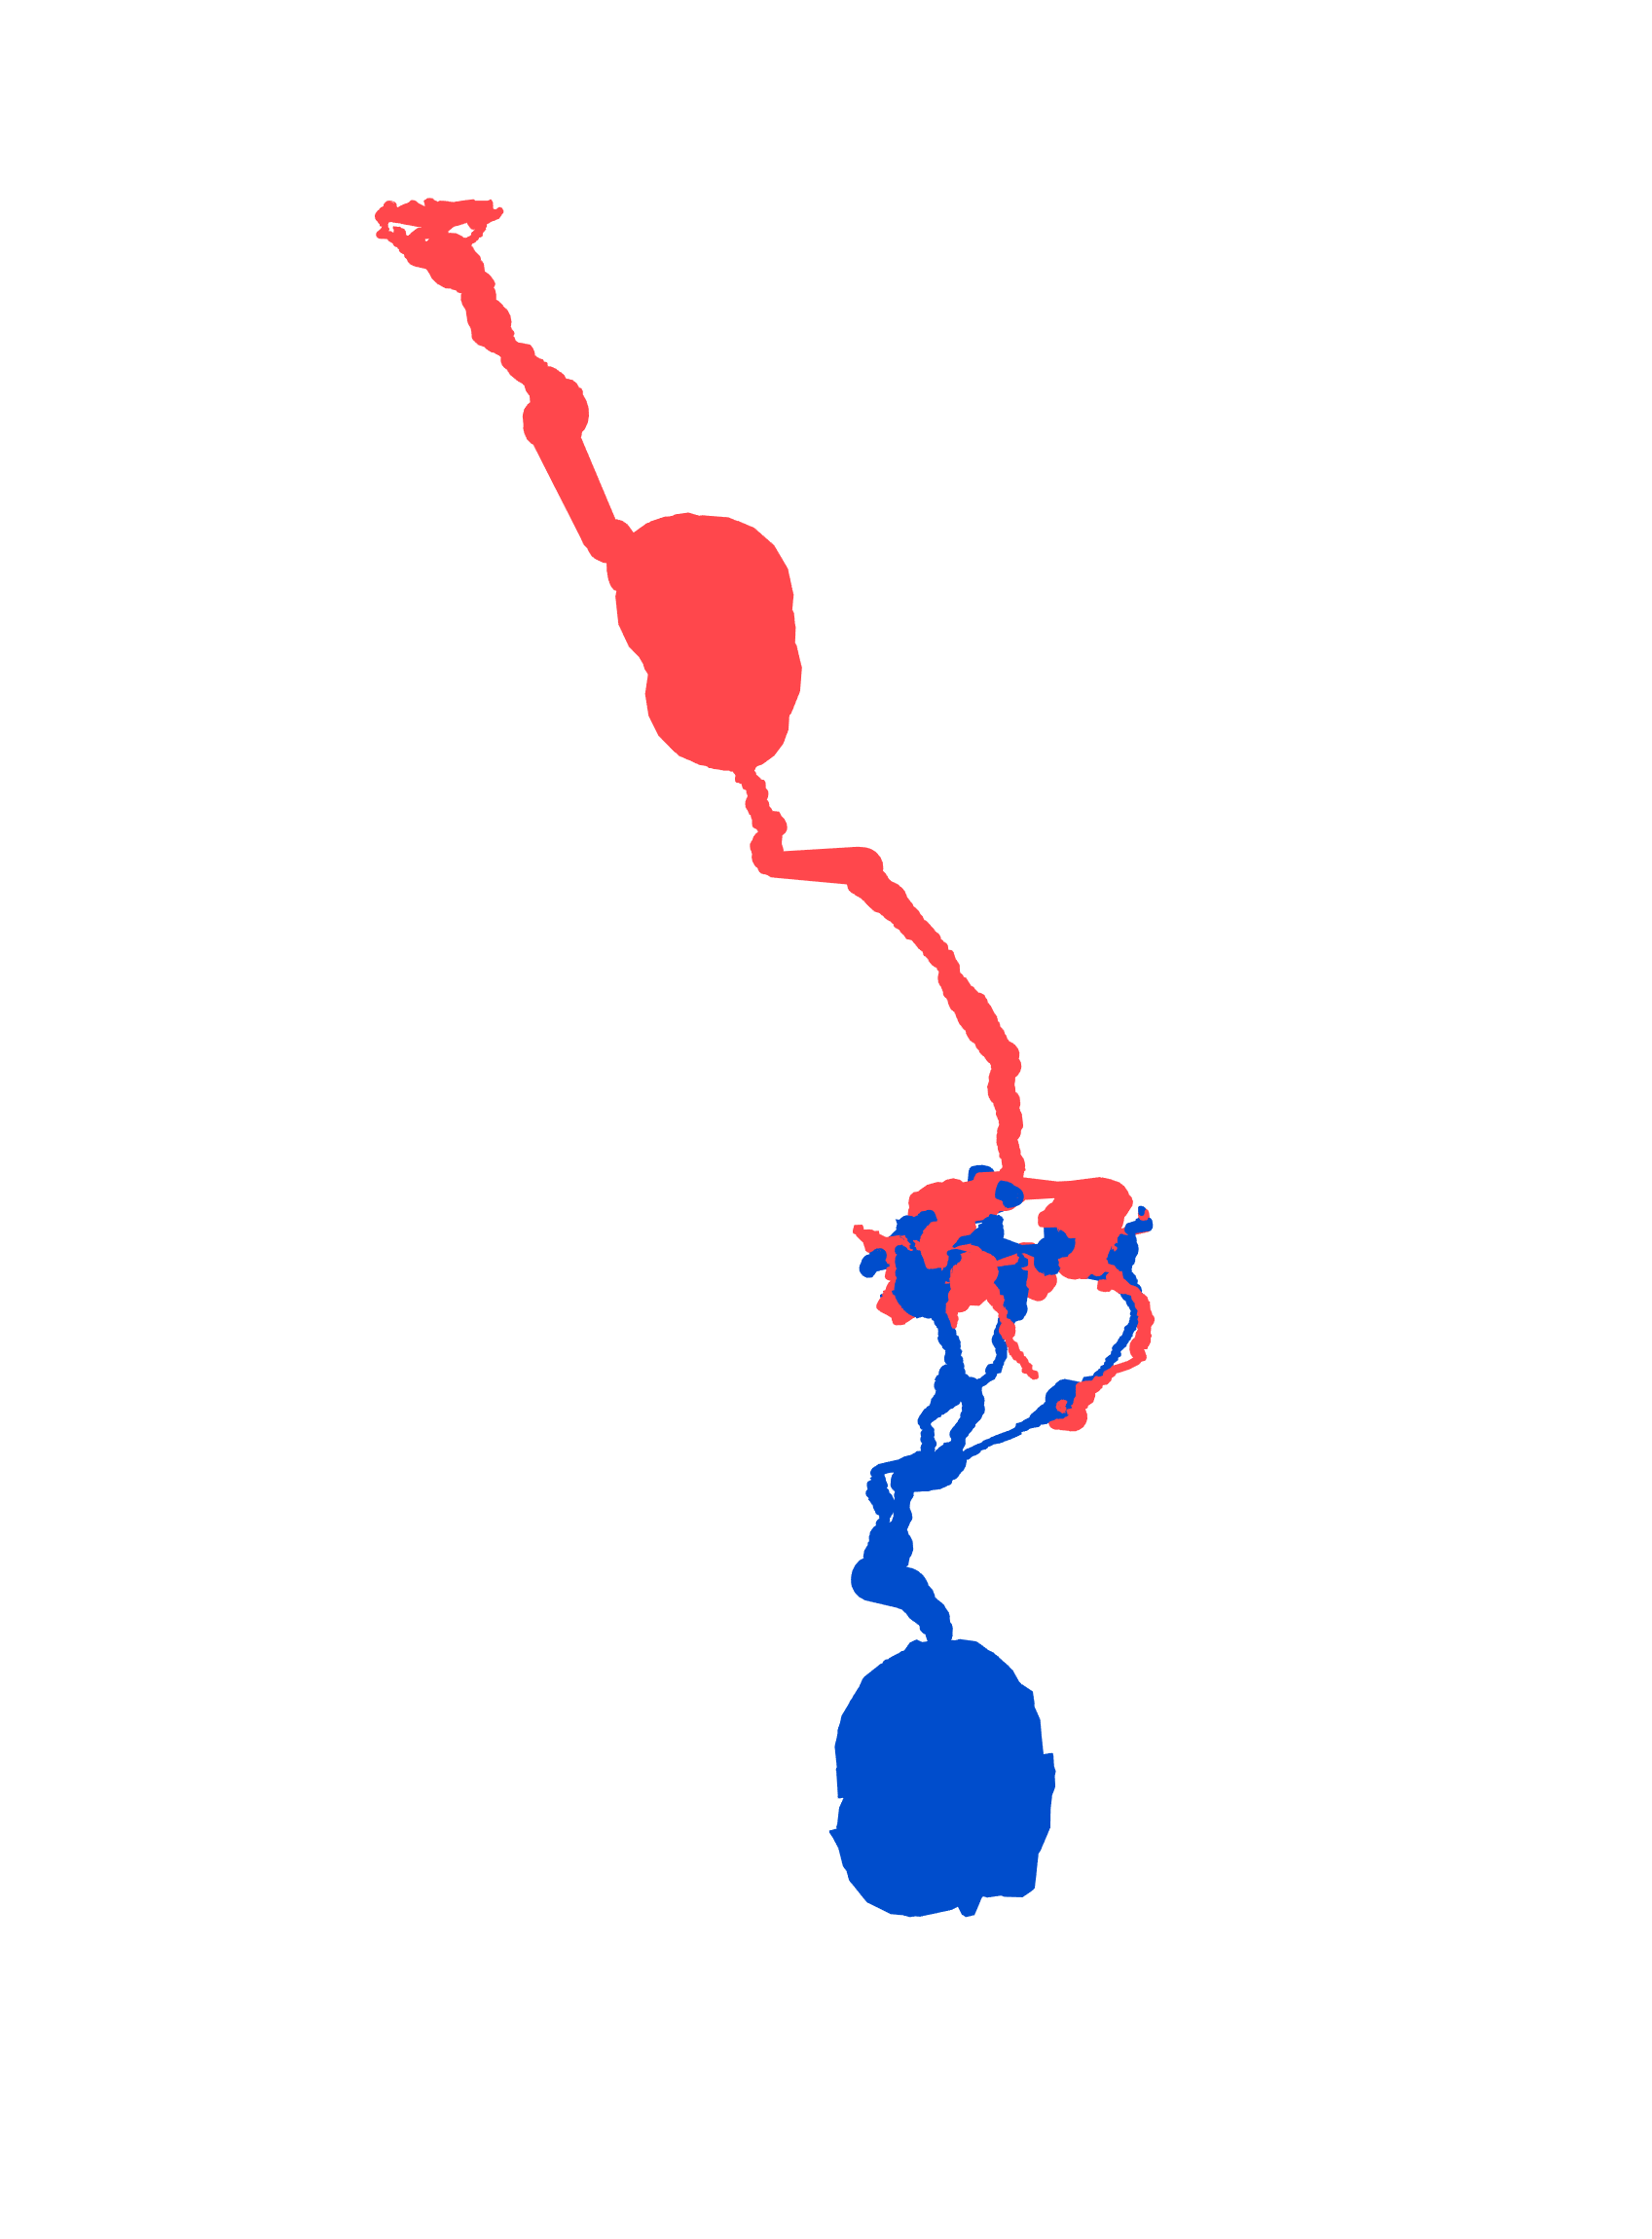
\includegraphics[width=\linewidth]{smidget_path}
	\end{wrapfigure}
	Rendering the above without any lighting creates a 3D figure with the appearance of a 2D projection.
	\begin{lstlisting}[language=matlab]
	% Turn off lighting for the active window
	lighting none;\end{lstlisting}
	This effect can also be accomplished in Blender with the following steps:
	\begin{enumerate}
		\item Switch from \texttt{Blender Render} to \texttt{Blender Game} on the top toolbar.
		\item On the \texttt{Material} tab under \texttt{Shading}, check the box for \texttt{Shadeless}. 
		\item On the bottom toolbar, using the button with a circle next to the \texttt{Object view} menu, switch from \texttt{Material} to \texttt{Texture} view.
		\item Click anywhere in the viewport, then press \texttt{N}. A menu should open to the right. Under \texttt{Shading}, check the \texttt{Shadeless} box.
	\end{enumerate}
	% -----------------------------------------------Subsection --
	\subsection{Volumetric Renders}
	% -----------------------------------------------Subsection --
	% --------------------------------------------Subsubsection -- 
	\subsubsection{Closed Curve}
	% --------------------------------------------Subsubsection --
	% -------------------------------------------------- Figure --
	\begin{wrapfigure}{r}{0.15\linewidth}
		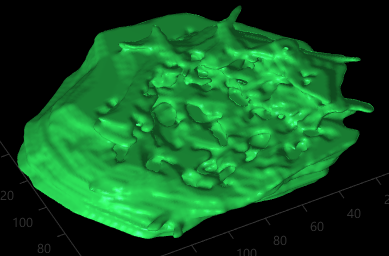
\includegraphics[width=\linewidth]{lmcone_render}
		\label{lmconeRender}
	\end{wrapfigure}
	% -------------------------------------------------- Figure -- 
	The closed curve render supports cutouts and multiple annotations per section. These renders lose their absolute position in the volume though. I hope to fix this soon. In the meantime, scenes with both ClosedCurve and Disc renders need to be aligned manually in Blender.
	\begin{lstlisting}[language=matlab]
	c2542 = Neuron(2542, 'i');
	% Specify ClosedCurve render
	c2542.build('closedcurve');
	% Smooth out the render by decreasing the sampling
	c2542.build('closedcurve', 'sampling', 0.8);
	% Use exportSceneDAE for Closed Curves
	exportSceneDAE(gca, 'c2542.dae');\end{lstlisting}
	
	% --------------------------------------------Subsubsection -- 
	\subsubsection{Disc Annotations}
	% --------------------------------------------Subsubsection --
	% -------------------------------------------------- Figure -- 
	\begin{wrapfigure}{r}{0.08\linewidth}
		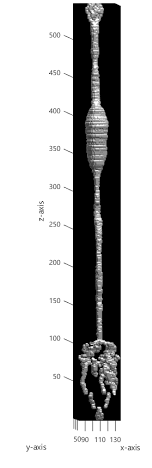
\includegraphics[width=\linewidth]{discBC}
		\label{discBC}
	\end{wrapfigure} 
	% -------------------------------------------------- Figure --
	The same method can be applied to Disc annotations as well for an accurate view of the annotations as discs in 3D. 
	
	As is, the result is not as good as the polygon mesh rendering, but could have some advantages in Blender. Right now I'm focusing on the polygon mesh renders for Disc annotations but may revisit this at some point.
	\begin{lstlisting}[language=matlab]
	% Load a rod bipolar cell
	c1893 = Neuron(1983, `i');
	% Build the 3D model (renders automatically)
	c1893.build('disc');
	
	% Adjust the resolution (default = 1)
	c1893.build('disc', 'sampling', 0.8);
	
	% Render a subset of sections
	c1893.build('disc', 'sections', 1100:1400);
	% Like the ClosedCurve renders, COLLADA export requires:
	exportSceneDAE(gca, 'filename.dae');\end{lstlisting}

	% -----------------------------------------------Subsection --
	\subsubsection{Image Traces}
	% -----------------------------------------------Subsection --
	Color outlines and transparent overlays can be extracted and rendered using the \texttt{volumeRender} function. See \ref{colorROI} for more information.
	% -----------------------------------------------Subsection --
	\subsection{Outlines}
	% -----------------------------------------------Subsection --

	Outlines of single closed curve annotations can also be added to a render using the \texttt{outline} option. I use this option for cone mosaics \ref{mosaicfig}
	
	\begin{lstlisting}[language=matlab]
	% Import an L/M-cone:
	c5751 = Neuron(5751, 'i');
	% Import a neighboring S-cone:
	c5752 = Neuron(5752, 'i');
	% Build the renders:
	c5751.build('outline');
	c5752.build('outline');
	% Plot both to the same figure
	c5751.render('EdgeColor', 'k');
	c5752.render('ax', gca,...
	'FaceColor', [0, 0.4, 1],...
	'FaceAlpha', 0.1,...
	'EdgeColor', [0, 0.4, 1]);\end{lstlisting}	
	% -------------------------------------------------- Figure --
	\begin{wrapfigure}{r}{0.2\linewidth}
		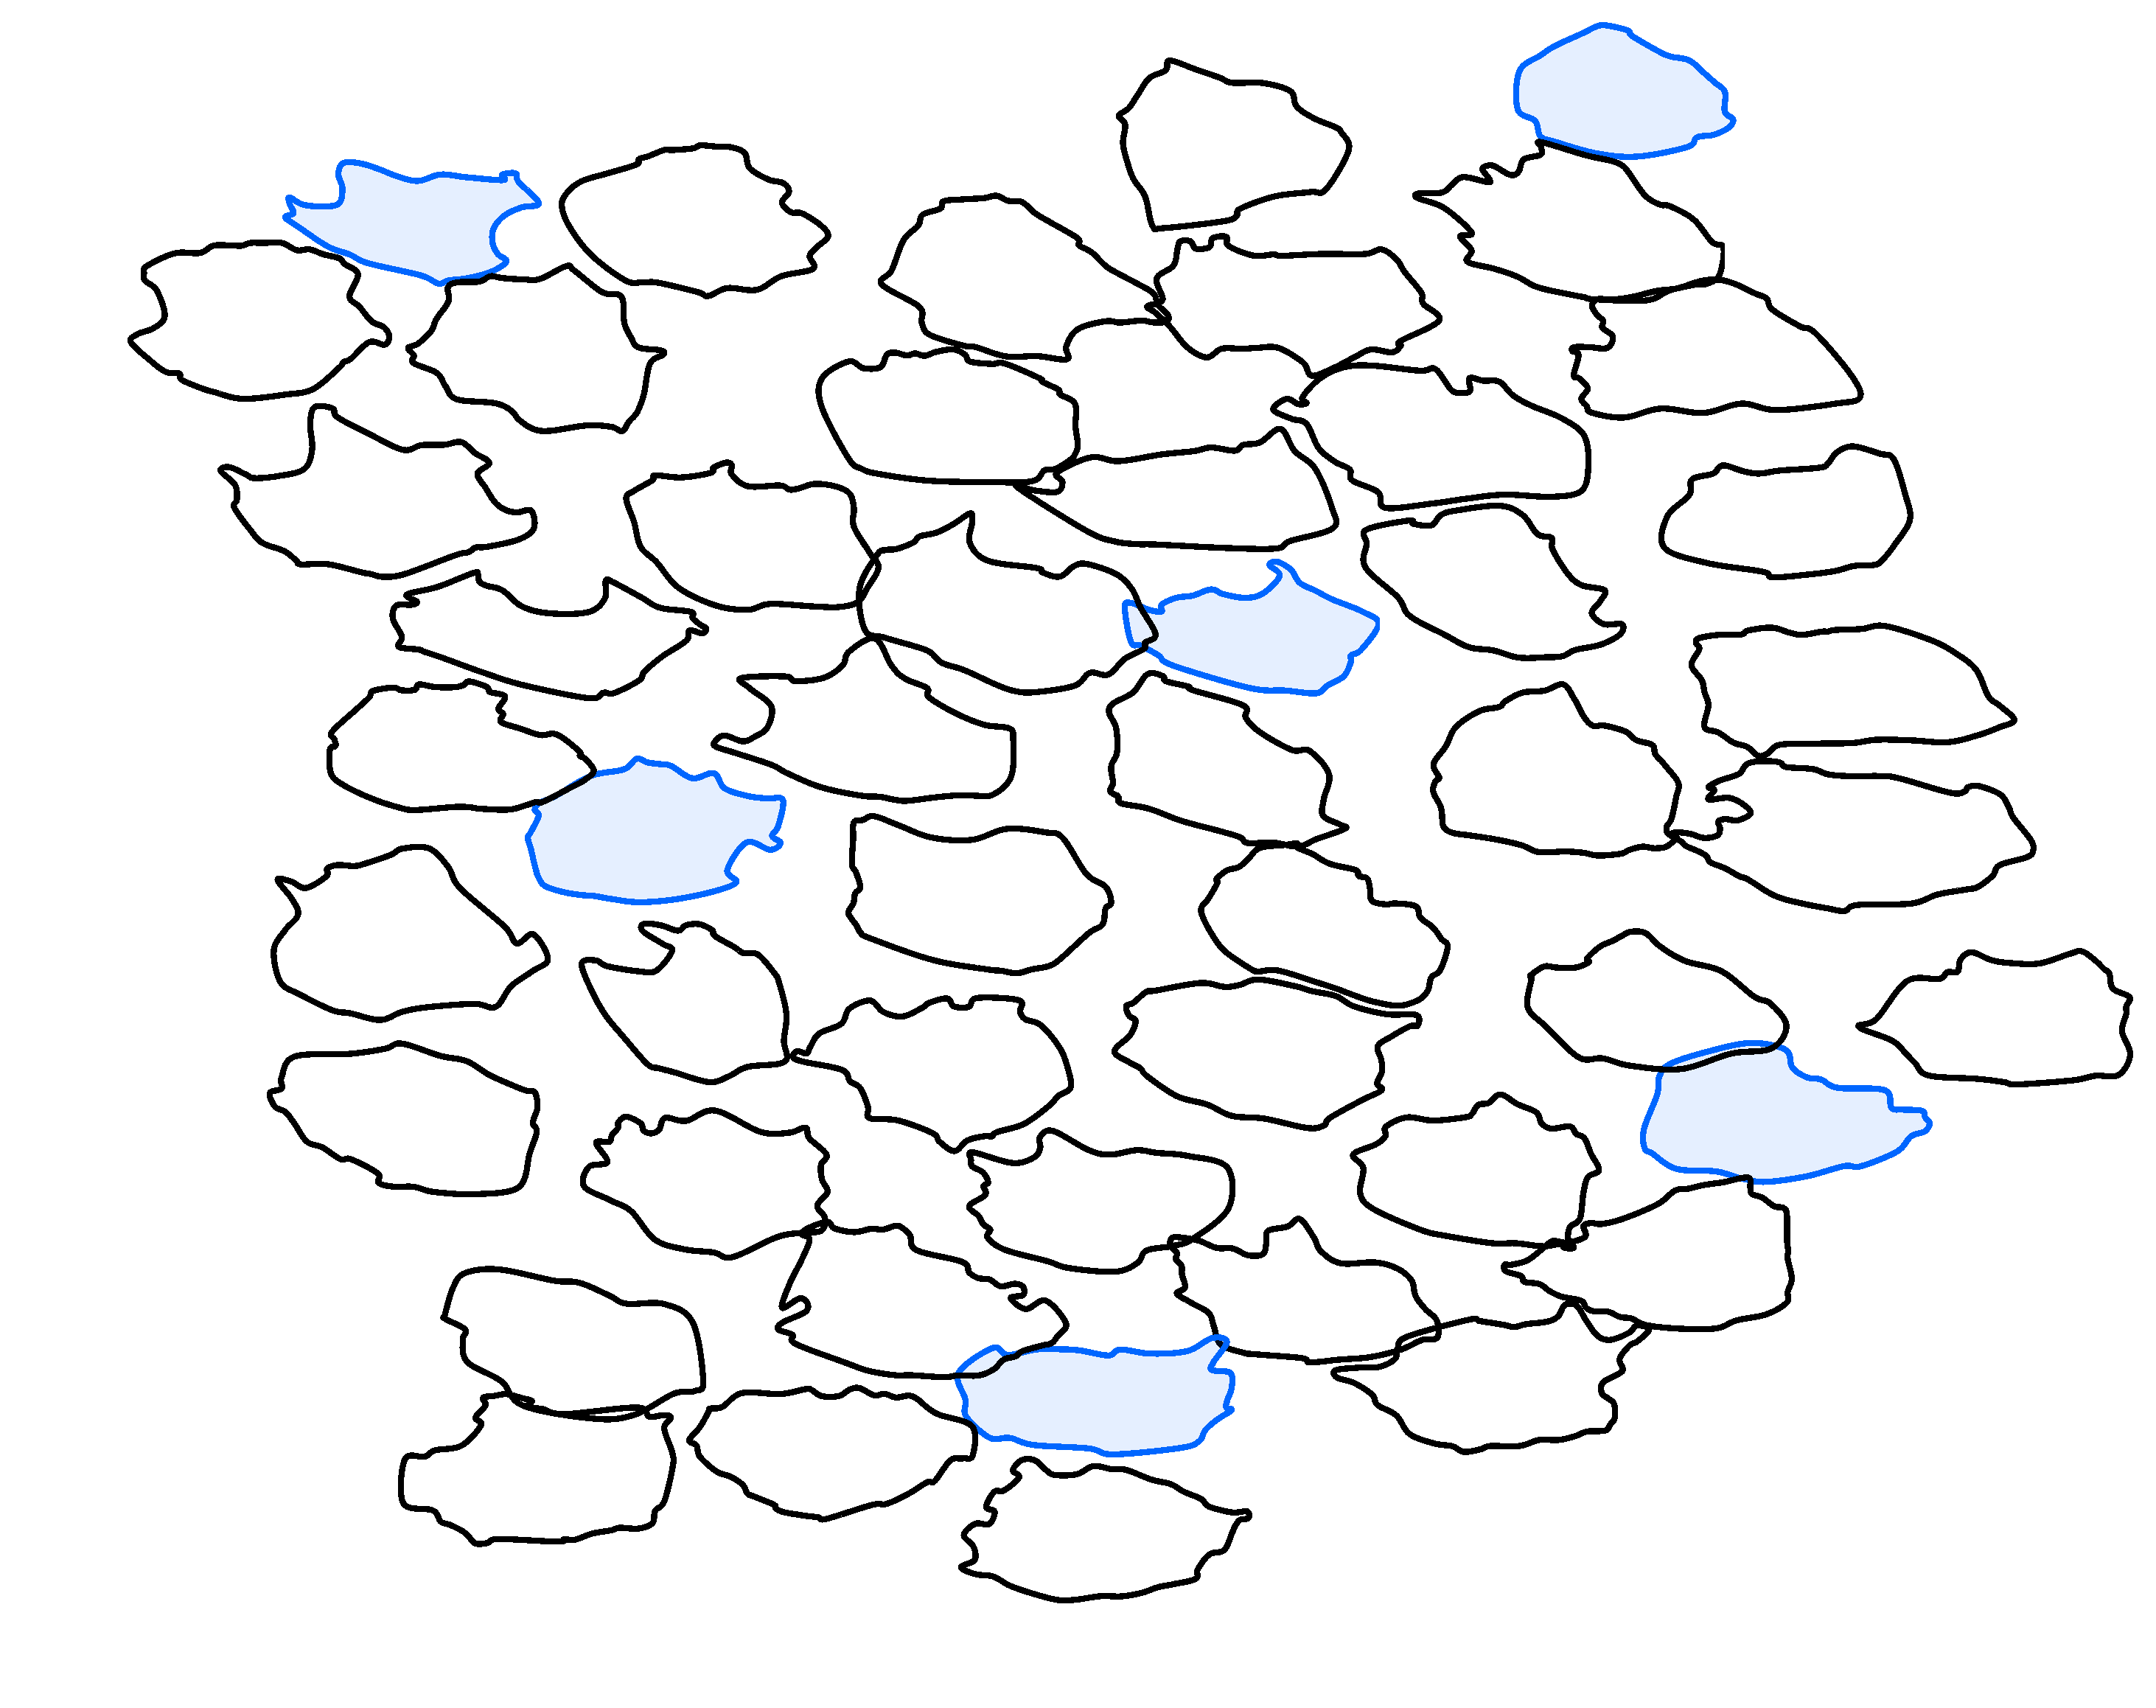
\includegraphics[width=\linewidth]{cone_mosaic}
		\label{mosaicfig}
	\end{wrapfigure}
		% -------------------------------------------------- Figure --
	% -----------------------------------------------Subsection -- 
	\subsection{VikingPlot}
	% -----------------------------------------------Subsection -- 
	Editing the MATLAB figure generated by VikingPlot can be a good alternative to Blender. A few useful commands:
	\begin{lstlisting}[language=matlab]
	% Make sure the figure is the active window.
	ax = gca; % Create a handle to the axis
	ax.Children % Returns a list of child structures
	% There should be PATCH and LIGHT objects.
	% Use numerical indexing to generate handles to the objects
	% NOTE: The numbering might be different on your figure
	lightObj = ax.Children(1);
	renderObj = ax.Children(2);
	% A few useful properties to edit for PATCH objects:
	renderObj.FaceColor = [0, 0.8, 0.3];
	renderObj.FaceAlpha = 0.7;\end{lstlisting}
	% ------------------------------------------------- Section -- 
	\section{Image Registration}
	% ------------------------------------------------- Section --
	% -------------------------------------------------- Figure -- 
	\begin{wrapfigure}{r}{0.25\linewidth}
		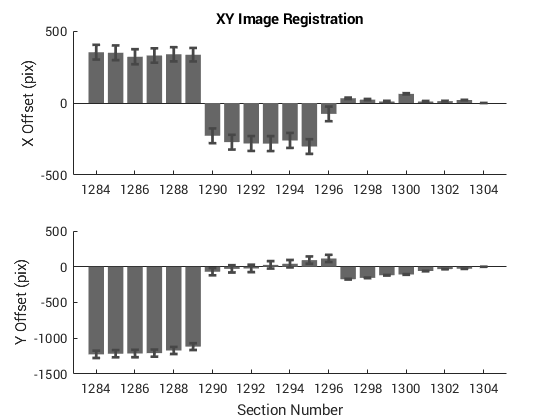
\includegraphics[width=\linewidth]{xyAlign}
	\end{wrapfigure}
	% -------------------------------------------------- Figure -- 
	% -----------------------------------------------Subsection -- 
	\subsection{Section Misalignment}
	% -----------------------------------------------Subsection --

	The function \texttt{xyRegistration.m} calculates the XY offset through a range of Z sections and outputs statistics on the offsets relative to the most sclerad section. 
	
	The first output is an Nx3 matrix (columns = Section Number, XOffset, YOffset). A data file tracks these offsets and can be updated using \texttt{updateRegistration.m}. The units are Viking's pixel coordinates. The transform is applied when the Neuron class first pulls X,Y coordinates from the OData service. This code is very new and needs quite a few improvements. However, the preliminary results are making a large difference in renders. See the code comments for more info.

	A second method is being used to bridge the gap between sections 915 (`above') and 936 (`below') in NeitzInferiorMonkey. The difference between the last annotation(s) at section 935 and the first annotation at section 915 is subtracted from all annotations above the gap. This is effective for midget RGCs but may need work for larger neurons with multiple branches crossing the gap.
	\begin{lstlisting}[language=matlab]
	[data, S] = xyRegistration('i', [1284 1309], true);
	updateRegistration('i', data);\end{lstlisting}
	% -----------------------------------------------Subsection --
	\subsection{IPL Boundary Markers}
	% -----------------------------------------------Subsection -- 
	% -------------------------------------------------- Figure -- 
	\begin{wrapfigure}{r}{0.2\linewidth}
		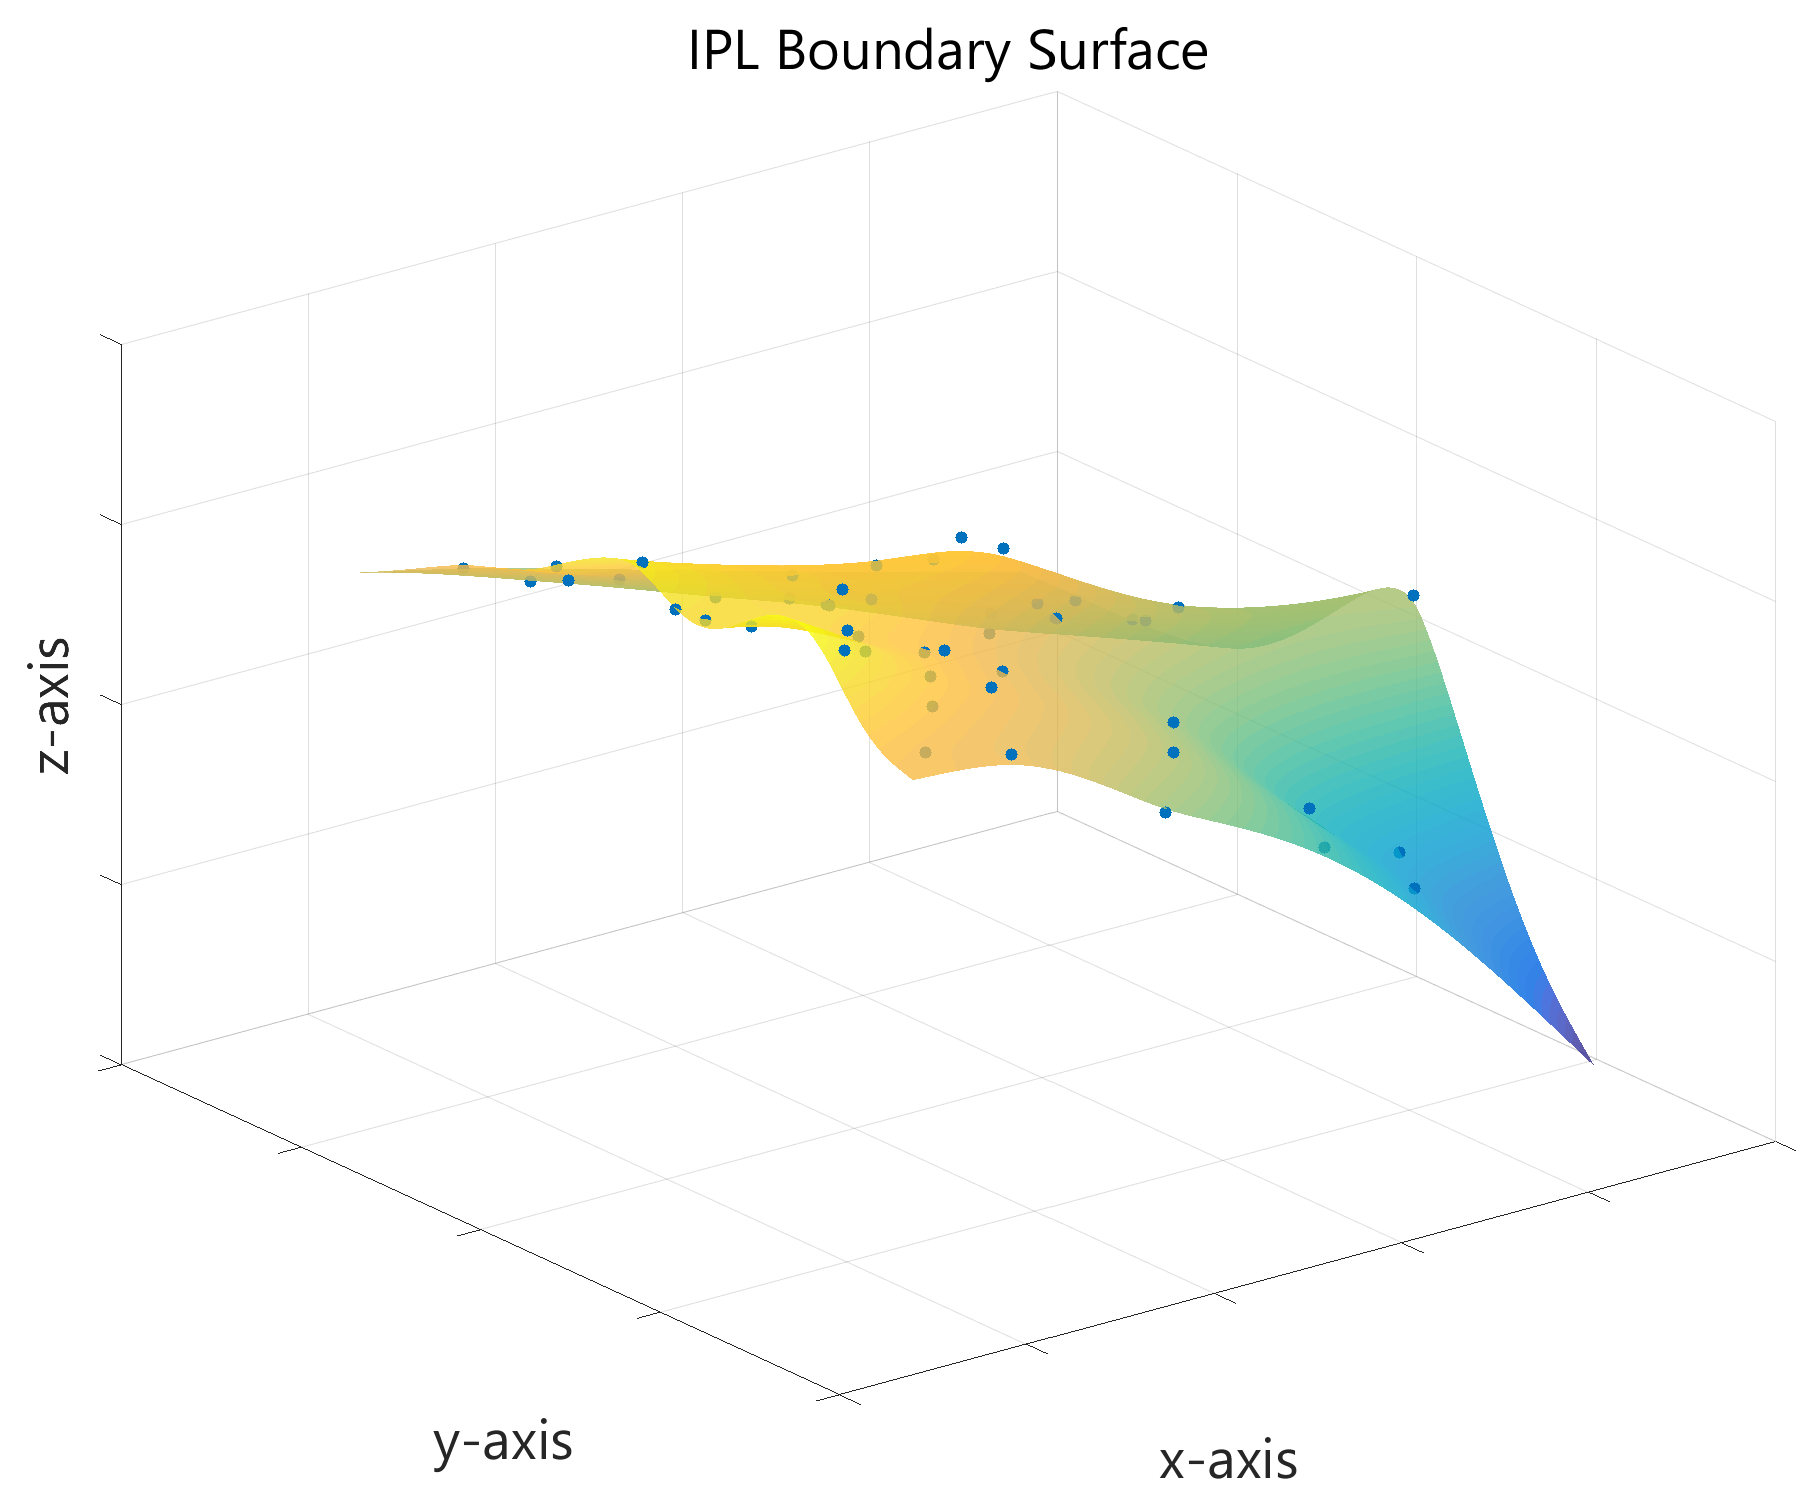
\includegraphics[width=\linewidth]{iplboundary}
		\label{iplboundary}
	\end{wrapfigure}
	% -------------------------------------------------- Figure -- 
	The INLBoundary and GCLBoundary objects retrieve all INL-IPL and IPL-GCL boundary markers, respectively. This can be used to create a surface representing the slope of the tissue. In the future, I will add a function for finding the nearest boundary markers to any given Neuron.
	\begin{lstlisting}[language=matlab]
	inl = INLBoundary('i');
	% Update marker locations from OData
	inl.update();
	% Create the surface
	inl.doAnalysis();
	% Plot the surface
	inl.plot();
	% Include the data points used to generate the surface
	inl.plot(true);\end{lstlisting}
	Warping the Z-axis to account for the gradually sloping tissue is a big goal. Soon I hope to have code to apply the transform - right now I'm thinking of adapting a commonly used method for warping neurons based on CHaT bands (\href{https://github.com/uygarsumbul/rgc}{Github repository}) \cite{Sumbul2014}.
	% ------------------------------------------------- Section -- 
	\section{Appendix}
	% ------------------------------------------------- Section --
	% -----------------------------------------------Subsection --
	\subsection{Matlab 101}\label{matlab101}
	% -----------------------------------------------Subsection --
	MATLAB tips are currently scattered throughout the documentation.. I am slowly consolidating them here.\\
	First, using SBFSEM-tools requires adding it to MATLAB's \href{https://www.mathworks.com/help/matlab/ref/addpath.html}{search path}. You'll need to fill in the `...' with the full file path where you cloned or downloaded sbfsem-tools.
	\begin{lstlisting}[language=matlab]
	addpath(genpath('C:\...\sbfsem-tools'));\end{lstlisting}
	The \texttt{addpath} command adds all the files in the specified folder to your search path. The \texttt{genpath} command adds all the sub-folders their files as well. If you're having trouble with this, there is a user interface (UI). This can be accessed by the \texttt{Set path} button on MATLAB's top toolbar, in the \texttt{Environment} panel. Make sure to click the \texttt{Add with subfolders} button (which is the equivalent of the \texttt{genpath} command). You can also open this UI by typing
	\begin{lstlisting}[language=matlab]
	pathtool;\end{lstlisting}
	into the command line.
	
	For any function or class, the \texttt{help} command will print information to the command line. For more information on MATLAB's functions, use \texttt{doc} command. To see the raw code, use the \texttt{edit} command.\\
	To explore any variable in a UI similar to Excel, use \texttt{openvar}. Most of the data types are user-defined classes like Neuron. A list of all the methods for any class can be obtained by \texttt{methods(className)}.
	\begin{lstlisting}[language=matlab]
	c127 = Neuron(127, 'i');
	% Open the variable in a UI
	openvar(c127);
	% These are the methods described in Section 3.2
	methods('Neuron')
	% Return the help for sbfsem.render.Cylinder
	help sbfsem.render.Cylinder
	% Go to matlab's documentation for tables
	doc table
	% See the cylinder code
	edit sbfsem.render.Cylinder\end{lstlisting}

	If you're planning on using SBFSEM-tools often, put the \texttt{addpath} code in your 
	\href{https://www.mathworks.com/help/matlab/ref/startup.html}{startup file} and it will run each time you open MATLABb. 
	% -----------------------------------------------Subsection --
	\subsection{Git 101}
	% -----------------------------------------------Subsection -- 
	Git can be downloaded \href{https://git-scm.com/}{here}. Once downloaded, you can open the terminal by right clicking anywhere in the whitespace of a File Explorer window and selecting \texttt{Git Bash here}. Do this in the folder you want sbfsem-tools to live in. 
	\begin{lstlisting}
	git clone http://github.com/sarastokes/sbfsem-tools.git\end{lstlisting}
	There should be a folder now called ``sbfsem-tools''. At any point, you can update the code to the latest version by right clicking on the folder itself, selecting \texttt{Git bash here} and typing in:
	\begin{lstlisting}
	git pull\end{lstlisting}
	This saves the step of deleting the existing sbfsem-tools folder and re-downloading it every time an update is available.
	% ------------------------------------------------- Section --	
	\begin{thebibliography}{[20]}
		\bibitem{borncg8} 
			BornCG Tutorial 8 - Smoothing and SubSurf\\
			\url{https://www.youtube.com/watch?v=gkN1aLaNWxk}
		\bibitem{isetbio}
			ISETBIO documentation format\\
			\url{https://github.com/isetbio/isetbio/wiki/Documentation-&-Formatting}
		\bibitem{Levy2009}
			Levy, B., Zhang, H. (2009) Spectral Mesh Processing. SIGGRAPH Asia Course Notes.
		\bibitem{Lorensen1987}
			Lorensen, W.E. \& Cline, H.E. (1987) Marching Cubes: A high resolution 3D surface reconstruction algorithm. \textit{Computer Graphics}, 21(4), 163-169
		\bibitem{Sumbul2014}
			Sumbul, U., Song, S., McCulloch, K., Becker, M., Lin, B., Sanes, J.R., Masland, R.H. \& Seung, H. S. (2014) A genetic and computation approach to structurally classify neuronal types. \textit{Nature Communications}, 5, 3512\\
			Github repository: \url{https://github.com/uygarsumbul/rgc}
		\bibitem{Zorin2000}
			Zorin, D. \& Schroder, P. (2000) Subdivision for modeling and animation. SIGGRAPH Course Notes
	\end{thebibliography}
\end{document}